
\subsection[Collections]{Object Collections}

% TODO: add picture of collections
\begin{frame}[fragile]
  \frametitle{Collections of Objects}
  \begin{itemize}
    \item Many problems have inherent order or structure
    \item Especially traditional `technical computing' problems
    \item Solution should use matching abstractions
    \item Arrays, lists, maps of parallel objects
    \item Specific segment of data, and associated computation and
      communication
    \item Need system support for efficient indexing
  \end{itemize}
\end{frame}

\begin{frame}[fragile]
  \frametitle{Collections of Objects: Concepts}
  \begin{itemize}
    \item Basic examples
      \begin{itemize}
      \item Matrix block
      \item Chunk of unstructured mesh
      \item Portion of distributed data structure
      \item Volume of simulation space
      \end{itemize}
      \pause
    \item Advanced Examples
      \begin{itemize}
      \item Abstract portions of computation
      \item Interactions among basic objects or underlying entities
      \end{itemize}
  \end{itemize}
\end{frame}

\begin{frame}[fragile]
  \frametitle{Collections of Objects}
  \begin{itemize}
    \item Structured: 1D, 2D, \ldots, 6D
    \item Unstructured: Anything hashable
      \pause
    \item Dense
    \item Sparse
      \pause
    \item Static - all created at once
    \item Dynamic - elements come and go
  \end{itemize}
\end{frame}

\begin{frame}[fragile]
  \frametitle{Collections of Objects: Communication}
  \begin{itemize}
    \item Point-to-point: to one element of a collection
    \item Broadcast: message to whole collection
    \item Multicast: message to subset of collection
    \item Reductions: message from (part of) collection
    \item Runtime system must provide efficient delivery for all
  \end{itemize}
\end{frame}

\begin{frame}[fragile]
  \frametitle{Collections of Objects: Runtime Service}
  \begin{itemize}
    \item System knows how to `find' objects efficiently: $(collection, index) \to processor$
    \item Applications can specify a mapping, or use simple
      runtime-provided options (e.g. blocked, round-robin)
    \item Distribution can be static, or dynamic!
    \item Key abstraction: application logic doesn't change, even
      though performance might
  \end{itemize}
\end{frame}

\begin{frame}[fragile]
  \frametitle{Collections of Objects: Runtime Service}
  \begin{itemize}
    \item Can develop and test logic in objects separately from their distribution
    \item Separation in time: make it work, then make it fast
    \item Division of labor: domain specialist writes object code, computationalist writes mapping
    \item Portability: different mappings for different systems, scales, or configurations
    \item Shared progress: improved mapping techniaues can benefit existing code
  \end{itemize}
\end{frame}




%% Object Collections: Supporting Data Decomposition (Phil)

%%     Motivate why object collections are needed
%%         simple adding numbers example
%%     Object Collections
%%         decompose data and associated work
%%         1/2/3D or more (eg: mesh chunk)
%%         dense / sparse (sparse solvers, collision detection)
%%         grow / shrink dynamically (AMR)
%%         each object exposes same functionality (methods)
%%         collection should be collectively addressable (method invocation on all objects)
%%         show sample pseudo-code snippets
%%     Object Collections: Collectives
%%     Examples
%%         simple scale a distributed vector (mcast)
%%         simple add array of numbers (mcast + redn)
%%         matrix vector product (mcast + gather)


\begin{frame}[fragile]
  \frametitle{Chare Array: Hello Example }
  \lstinputlisting{code/arrayHello.ci}
\end{frame}

\begin{frame}[fragile]
  \frametitle{Chare Array: Hello Example }
  \lstinputlisting[basicstyle=\scriptsize]{code/arrayHello.cpp}
\end{frame}

\begin{frame}[fragile]
   \frametitle{Hello World Array Projections Timeline View}\scriptsize
  \begin{itemize}
    \item Add \texttt{-tracemode projections} to link line to enable tracing
    \item Run Projections tool to load trace log files and visualize performance
  \end{itemize}
  \begin{center} 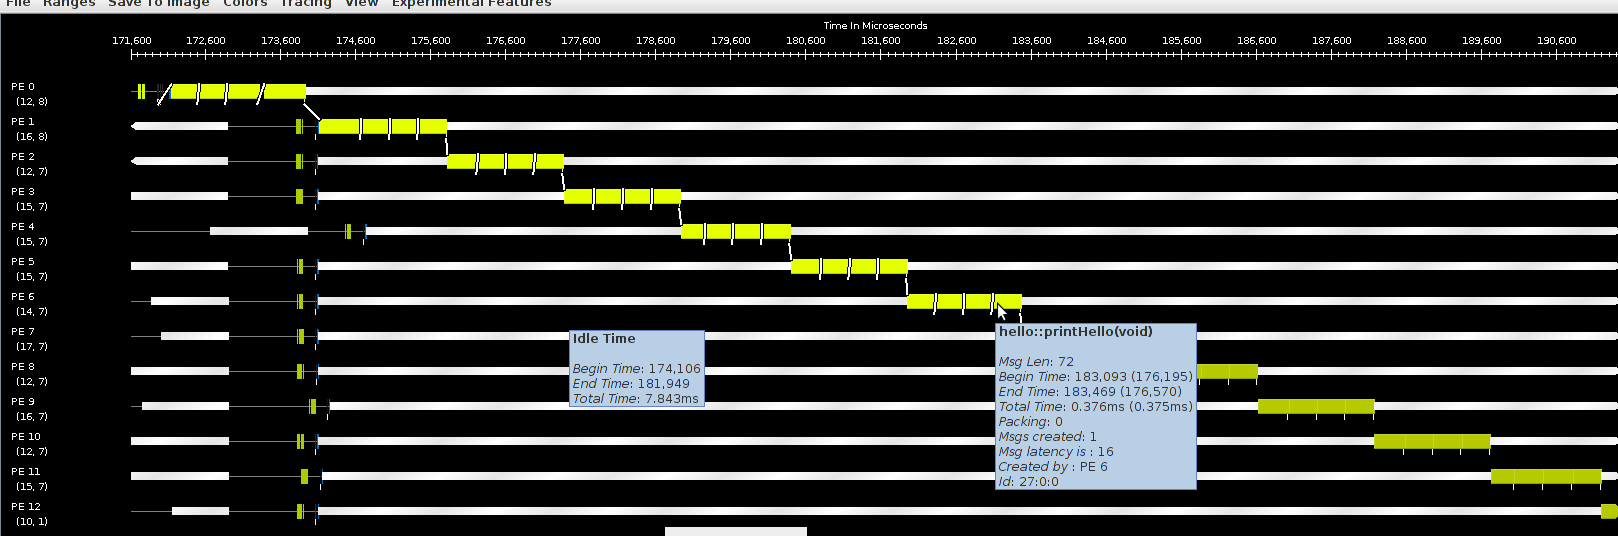
\includegraphics[width=0.99\textwidth]{figures/arrayHelloTimeline} \end{center}
  \begin{itemize}
   \item arrayHello on BG/Q 16 Nodes, mode c16, 1024 elements (4 per process)
  \end{itemize}
\end{frame}






\begin{frame}[fragile]
  \frametitle{Declaring a Chare Array}
  \texttt{.ci} file:
  \begin{lstlisting}
    array [1d] foo {
      entry foo(); // constructor
      // ... entry methods ...
    }
    array [2d] bar {
      entry bar();  // constructor
      // ... entry methods ...
    }
  \end{lstlisting}
  \texttt{.C} file:

  \begin{lstlisting}
    struct foo : public CBase_foo {
      foo() { }
      foo(CkMigrateMessage*) { }
      // ... entry methods ...
    };
    struct bar : public CBase_bar {
      bar() { }
      bar(CkMigrateMessage*) { }
      // ... entry methods ...
    };
  \end{lstlisting}
\end{frame}

\begin{frame}[fragile]
  \frametitle{Constructing a Chare Array}
  \begin{itemize}
    \item Constructed much like a regular chare
    \item The size of each dimension is passed to the constructor
  \end{itemize}
  \begin{lstlisting}
    void someMethod() {
       CProxy_foo::ckNew(10);
       CProxy_bar::ckNew(5, 5);
    }
  \end{lstlisting}
  \begin{itemize}
  \item The proxy may be retained:
  \end{itemize}
  \begin{lstlisting}
    CProxy_foo myFoo = CProxy_foo::ckNew(10);
  \end{lstlisting}
  \begin{itemize}
  \item The proxy represents the entire array, and may be indexed to obtain a
    proxy to an individual element in the array
  \end{itemize}
  \begin{lstlisting}
    myFoo[4].invokeEntry();
  \end{lstlisting}
\end{frame}

\begin{frame}[fragile]
  \frametitle{\code{thisIndex}}
  \begin{itemize}
  \item 1d: \code{thisIndex} returns the index of the current chare array element
  \item 2d: \code{thisIndex.x} and \code{thisIndex.y} returns the indices of
    the current chare array element
  \end{itemize}
  \texttt{.ci} file:
  \begin{lstlisting}
    array [1d] foo {
      entry foo();
    }
  \end{lstlisting}

  \texttt{.C} file:
  \begin{lstlisting}
    struct foo : public CBase_foo {
      foo() {
        CkPrintf("array index = %d", thisIndex);
      }
    };
  \end{lstlisting}

\end{frame}

\removeForTutorial{
\begin{frame}[fragile]
  \frametitle{Chare Array: Hello Example }
  \lstinputlisting{code/arrayHello.ci}
\end{frame}

\begin{frame}[fragile]
  \frametitle{Chare Array: Hello Example }
  \lstinputlisting[basicstyle=\scriptsize]{code/arrayHello.cpp}
\end{frame}

\begin{frame}[fragile]
   \frametitle{Hello World Array Projections Timeline View}\scriptsize
  \begin{itemize}
    \item Add \texttt{-tracemode projections} to link line to enable tracing
    \item Run Projections tool to load trace log files and visualize performance
  \end{itemize}
  \begin{center} 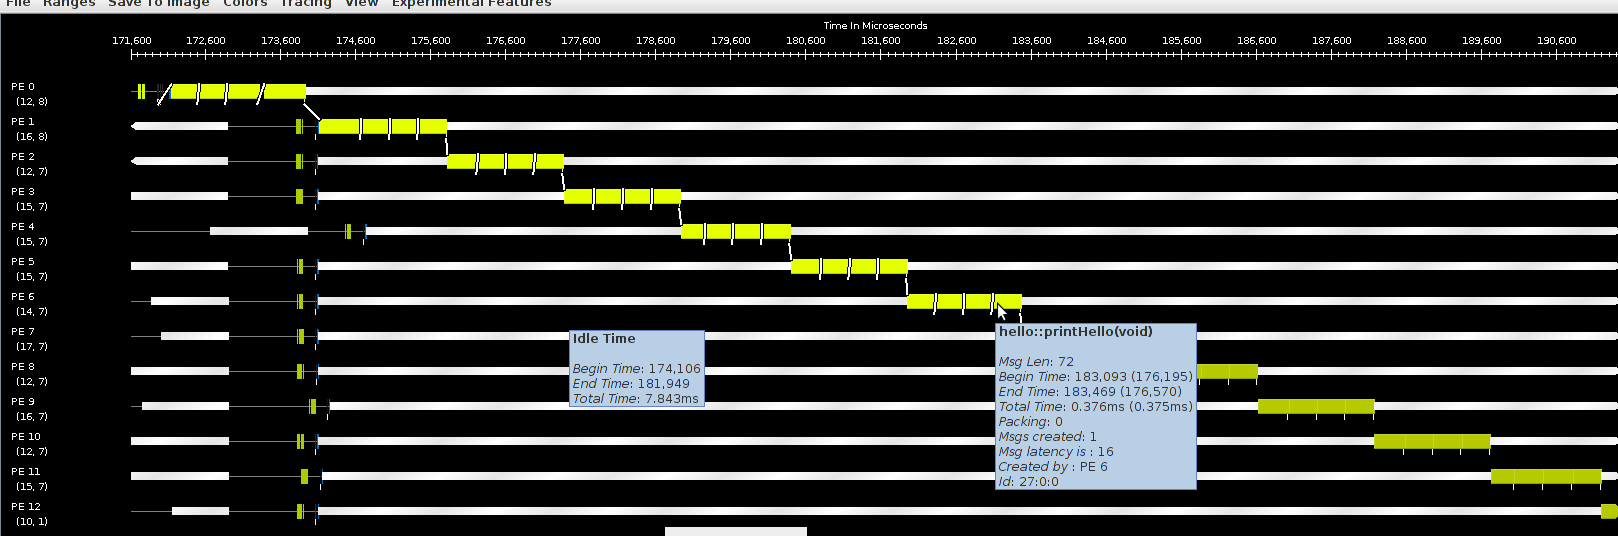
\includegraphics[width=0.99\textwidth]{figures/arrayHelloTimeline} \end{center}
  \begin{itemize}
   \item arrayHello on BG/Q 16 Nodes, mode c16, 1024 elements (4 per process)
  \end{itemize}
\end{frame}



}

\begin{frame}[fragile]
  \frametitle{Collections of Objects: Runtime Service}
  \begin{itemize}
    \item System knows how to `find' objects efficiently: $(collection, index) \to processor$
    \item Applications can specify a mapping, or use simple
      runtime-provided options (e.g. blocked, round-robin)
    \item Distribution can be static, or dynamic!
    \item Key abstraction: application logic doesn't change, even
      though performance might
  \end{itemize}
\end{frame}

\begin{frame}[fragile]
  \frametitle{Collections of Objects: Runtime Service}
  \begin{itemize}
    \item Can develop and test logic in objects separately from their distribution
    \item Separation in time: make it work, then make it fast
    \item Division of labor: domain specialist writes object code, computationalist writes mapping
    \item Portability: different mappings for different systems, scales, or configurations
    \item Shared progress: improved mapping techniques can benefit existing code
  \end{itemize}
\end{frame}

\begin{frame}[fragile]
  \frametitle{Collections of Objects}
  \begin{center}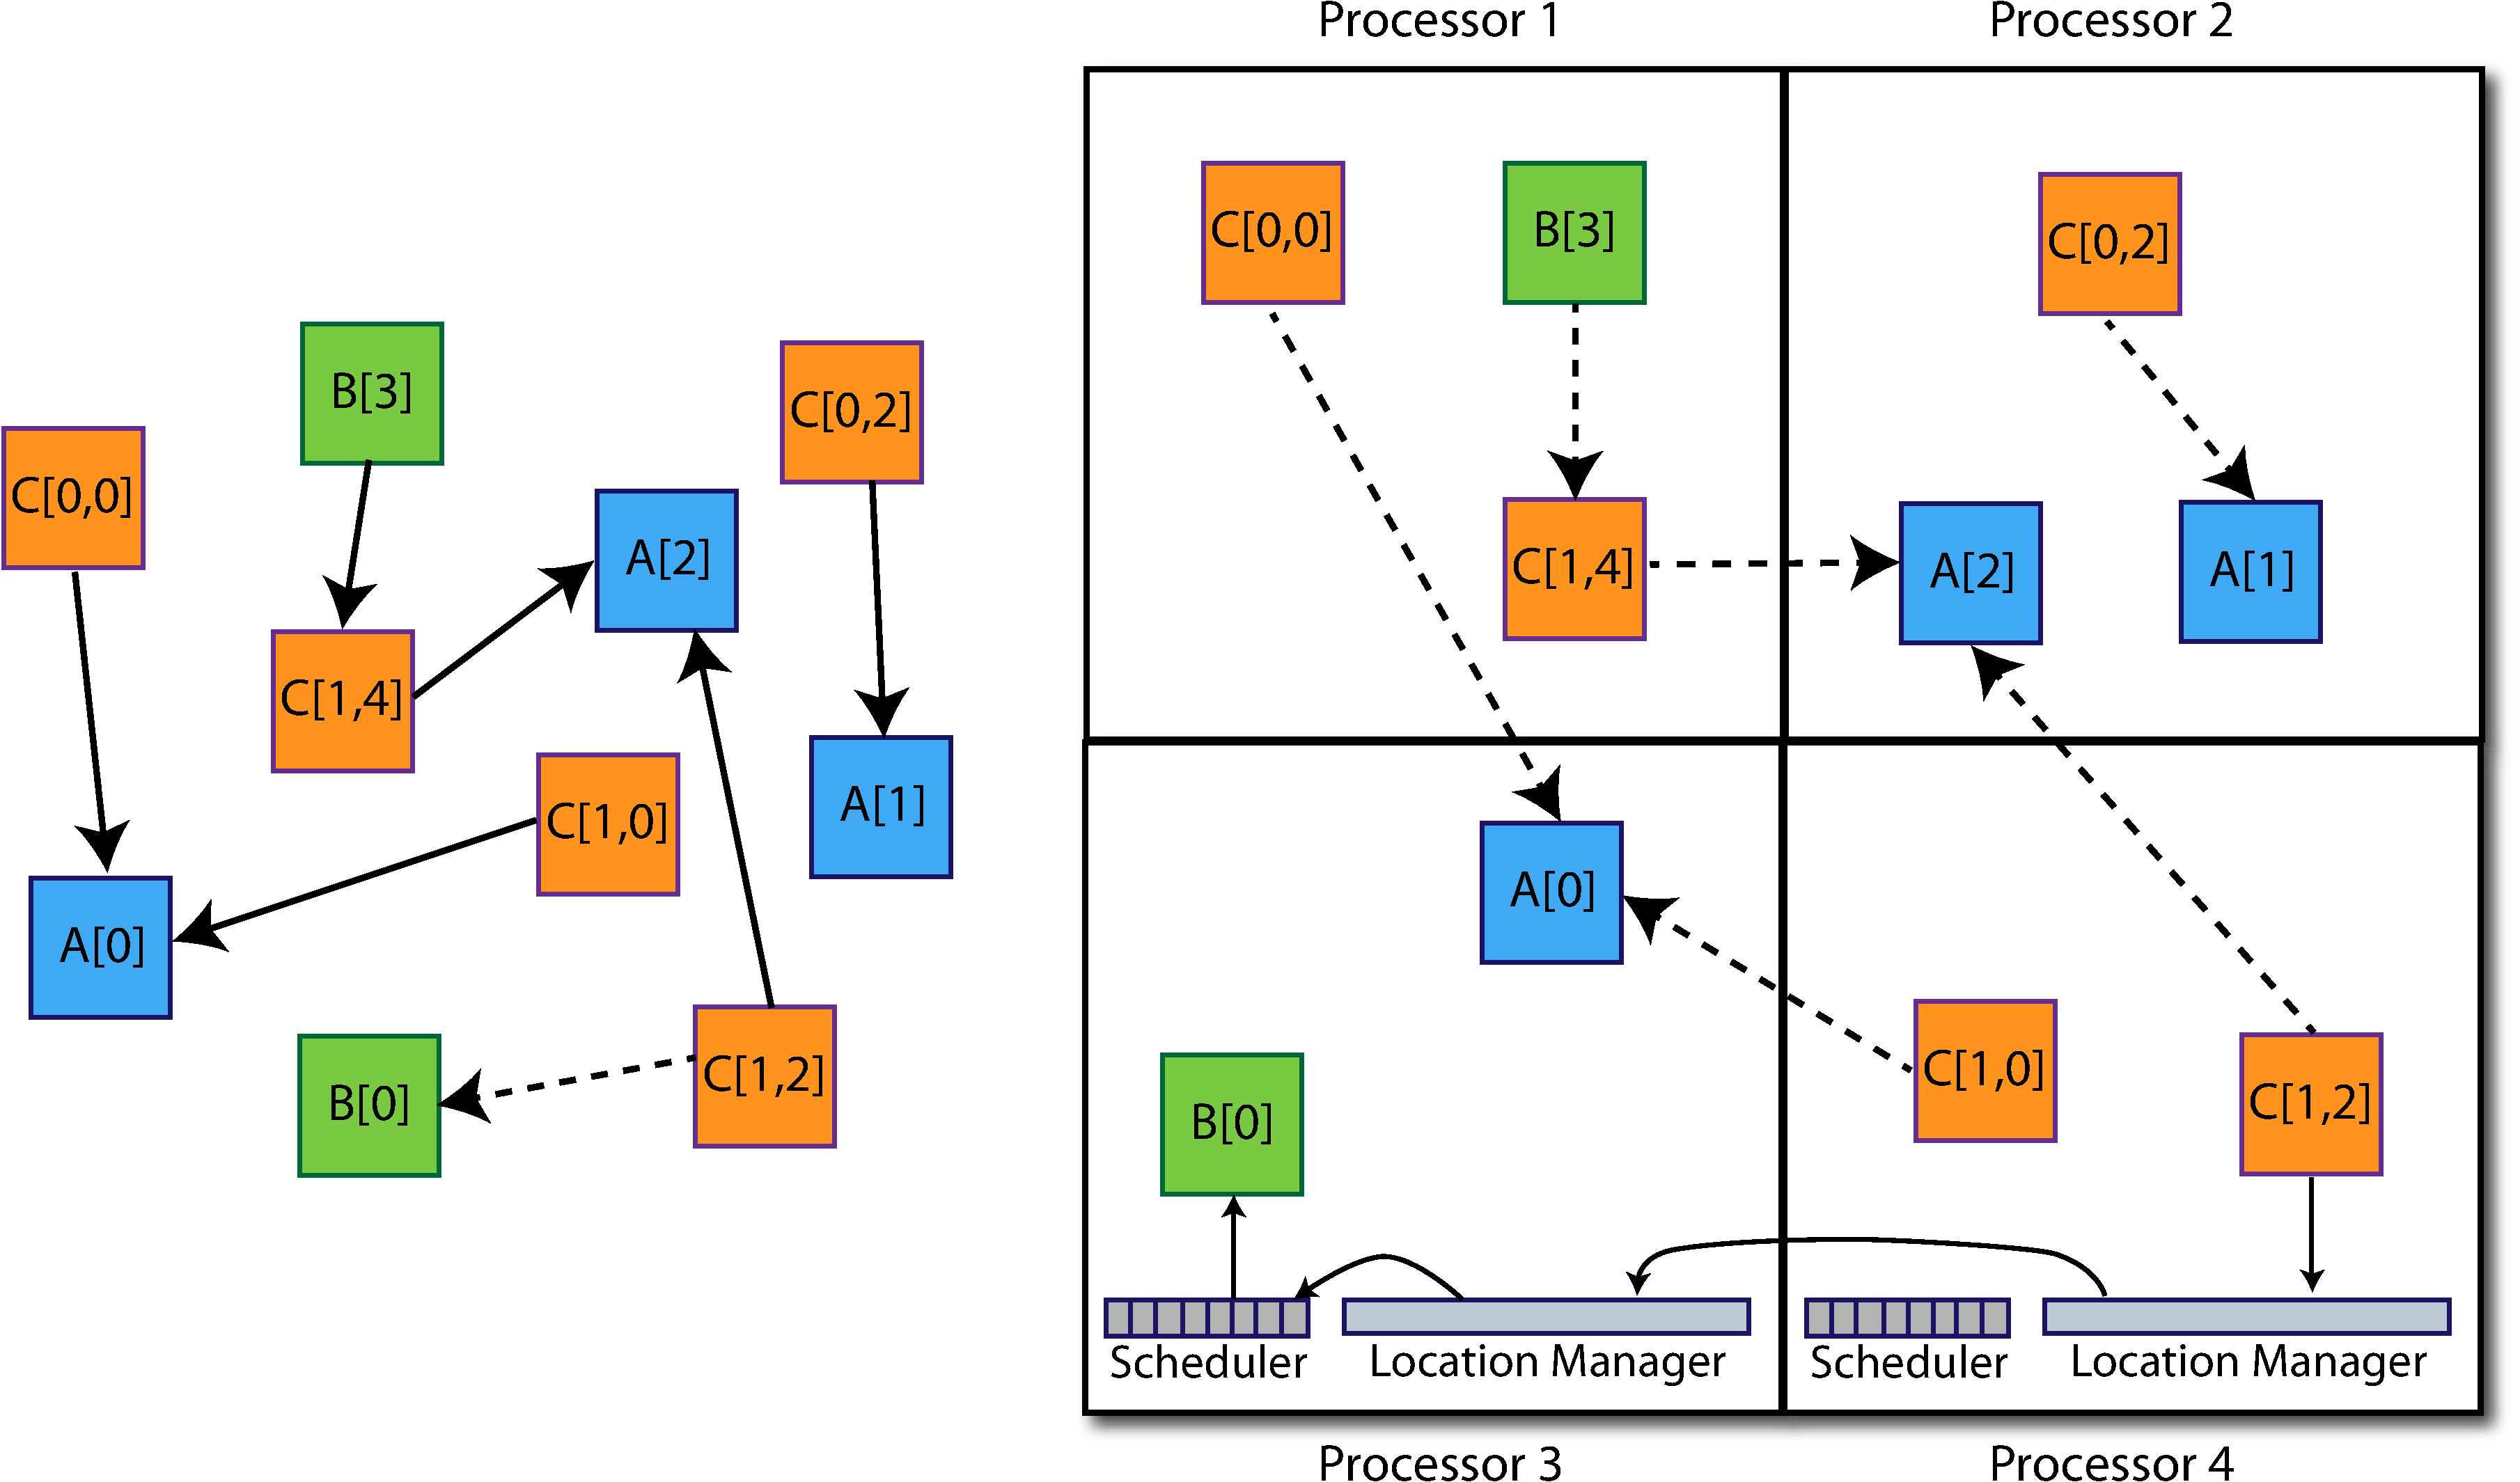
\includegraphics[width=0.9\textwidth]{figures/elements2.pdf}\end{center}
\end{frame}

\begin{frame}[fragile]
  \frametitle{Collective Communication Operations}
  \begin{itemize}
    \item Point-to-point operations involve only two objects
    \item Collective operations that involve a collection of objects
    \item Broadcast: calls a method in each object of the array
    \item Reduction: collects a contribution from each object of the array
    \item A spanning tree is used to send/receive data
  \end{itemize}
    \begin{center} 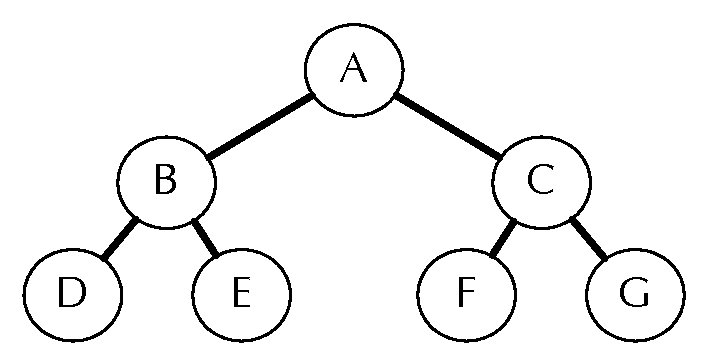
\includegraphics[width=0.5\textwidth]{figures/spanningTree.pdf} \end{center}
\end{frame}


\begin{frame}[fragile]
  \frametitle{Broadcast}
  \begin{itemize}
    \item A message to each object in a collection
    \item The chare array proxy object is used to perform a broadcast
    \item It looks like a function call to the proxy object
    \item From the main chare:
    \begin{lstlisting}
CProxy_Hello helloArray = CProxy_Hello::ckNew(helloArraySize);
helloArray.foo();
    \end{lstlisting}
    \item From a chare array element that is a member of the same array:
     \begin{lstlisting}
 thisProxy.foo()
    \end{lstlisting}
    \item From any chare that has a proxy \texttt{p} to the chare array
      \begin{lstlisting}
 p.foo()
      \end{lstlisting}
  \end{itemize}
\end{frame}

\begin{frame}[fragile]
  \frametitle{Reduction}
  \begin{itemize}
  \item Combines a set of values: sum, max, aggregate
  \item Usually reduces the set of values to a single value
  \item Combination of values requires an operator
  \item The operator must be commutative and associative
  \item Each object calls \code{contribute} in a reduction
  \end{itemize}
\end{frame}

\begin{frame}[fragile]
  \frametitle{Reduction: Example}
  \lstinputlisting{code/reductionMainTarget.ci}
\end{frame}

\begin{frame}[fragile]
  \frametitle{Reduction: Example}
  \lstinputlisting[basicstyle=\tiny]{code/reductionMainTarget.cpp}
Output:
  \begin{lstlisting}[basicstyle=\tiny]
value: 1176
Program finished.
  \end{lstlisting}
\end{frame}

\removeForClass{
\begin{frame}[fragile]
  \frametitle{Quick Hands-on}
  \begin{itemize}
  \item Log onto your vesta account.
  \item Obtain the following code:\\ git clone git://charm.cs.uiuc.edu/users/tutorial\_exercise
  \item Read the README.
  \item Change to toy directory, and read assignment.txt.
  \item Uncomment the CHARMC declaration at top of Makefile and make.
  \item ./charmrun -A $<$your\_account$>$ +p4 ./hello 16.
  \item Modify paramter to be an array instead of int.
  \end{itemize}
\end{frame}
}

%comment for removeForClass macro to work
